%!TEX root = main-doc.tex
%
% File: methodology.tex
%
% Date: ? 
%
% Description:
%   
%
%
\chapter{Methodology} \label{chap:methodology}
\vspace{-1cm}
\summary{Based on the literature review in Chapter \ref{chap:background}, it is evident that the extendibility of multidimensional sparse arrays is an incredibly important topic that has been overlooked, specifically with regards to data warehousing and OLAP. In order to make a contribution to this field, an extendible multidimensional sparse array model must be developed, implemented and evaluated. This chapter presents the proposed model design and experimental procedures for the research study.}

%%%%%%%%%%%%%%%%%%%%%%%%%%%%%%%%%%%%%%%%%%%%%%%%%%%%%%%%%%%%%%%%%%%%%%%%%%%%%%%%
\section{Extendible Multi-Dimensional Sparse Arrays}

In order to represent a data warehouse in a multidimensional space a formula needs to be defined to increase the dimensionality of the storage scheme without changing the mapping function f(). As sparse data warehouses consist of large quantities of information with few non-zero elements, an efficient storage scheme that represents these non-zero elements must be chosen. Furthermore a method for extendibility of the multi-dimensional sparse array representation must be chosen.

%%%%%%%%%%%%%%%%%%%%%%%%%%%%%%%%%%%%%%%%%%%%%%%%%%%%%%%%%%%%%%%%%%%%%%%%%%%%%%%%
\subsection{Multi-Dimensional Sparse Array Representation}
In order to improve the storage efficiency of multi-dimensional sparse arrays, a good storage scheme must be chosen. A comparison of the different sparse array storage techniques detailed in Section \ref{chap:background} is carried out.

CRS and CCS are both only used for 2-dimensional arrays. In the work of Goil et al. \cite{goil:bess} it is clear that BESS out performs Offset-Value pair. In the work of Wang \cite{wang:2014sar} it is evident that although PTCS has a better storage ratio and xCRS/xCCS and BxCRS have faster element retrieval times, BESS has a faster construction time and a faster multi-dimensional aggregation time than all of the other storage schemes. 

BESS is a very simple and efficient multi-dimensional sparse array representation as it maps a multi-dimensional sparse array space to a one-dimensional array space, resulting in a bit encoded key index \cite{wang:2014sar}.

A multi-dimensional sparse array data model using a BESS array representation scheme as well as a model using a CRS representation scheme will be analysed.
%%%%%%%%%%%%%%%%%%%%%%%%%%%%%%%%%%%%%%%%%%%%%%%%%%%%%%%%%%%%%%%%%%%%%%%%%%%%%%%%
%\subsection{Extendible Multi-Dimensional Array Representation}
%In order to improve the performance of extendible multi-dimensional arrays, chunking techniques are used.

%%%%%%%%%%%%%%%%%%%%%%%%%%%%%%%%%%%%%%%%%%%%%%%%%%%%%%%%%%%%%%%%%%%%%%%%%%%%%%%%
\subsection{Extendible Multi-Dimensional Sparse Array Representation}

\textbf{NB - Still working on this section}

 By making use of chunking techniques on a BESS array representation scheme as well as a CRS array representation scheme. The proposed extendibility model can increase the dimensionality of the storage scheme by either increasing the density of the array or increasing the dimension  of the indices or bounds of the array. When increasing a sparse array by density, the bounds and structure remain the same, new elements are slot into a chunk where there was a free space. Two algorithms will need to be developed and implemented in software in order to determine which algorithm performs better.
 
 To assess the performance of the extendible multi-dimensional models, a measure of the storage efficiency and order of retrieval of queries shall be conducted using basic construction, low level retrieval and partial match query array operations.
 
 The two algorithms will be tested on a 2D array (both CRS and BESS), a 3D array(only BESS) and a 4D array(Only BESS) to asses their limitations on different dimensionalities.
 
 Figure \ref{fig:proposedmethod} shows the main steps in the proposed methodology.

 
 \begin{figure}
 	\centering
 	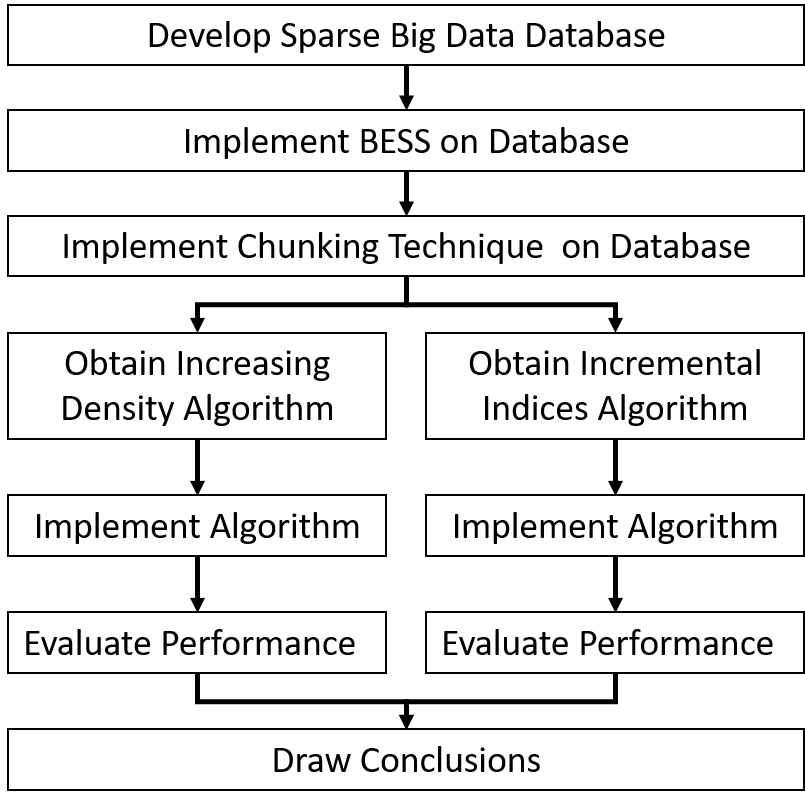
\includegraphics[width=0.7\linewidth]{proposedMethod}
 	\caption{Proposed Methodology}
 	\label{fig:proposedmethod}
 \end{figure}
 